\chapter{Index}

record存储在底层页面上，如果按照堆模型，要找到某个record，需要遍历整个页面，时间复杂度为$O(n)$，考虑到io非常慢，这个复杂度是难以接受的。一个完整的存储引擎，一般包括三部分的内容：底层存储组织、索引结构和缓冲管理。本章介绍索引结构，主要包括btree和lsm\cite{o1996log}结构。

\section{索引概念}

抽象上看，一个索引就是一个函数，给定key，输出record的位置。
$$
pos = f(key)
$$
将问题简化，假设一个堆模型上，record的位置不发生变化，如何表达这个函数$f(x)$？一个简单的方案是采用用数组记录每个record的位置，如\figurename\ref{fig:3-heap}所示。为了快速找到某个record的位置，需要将数组按照key顺序排列，然后以二分搜索在数组上定位，这个复杂度为$O(log(n))$。

\begin{figure}[H]
    \centering
    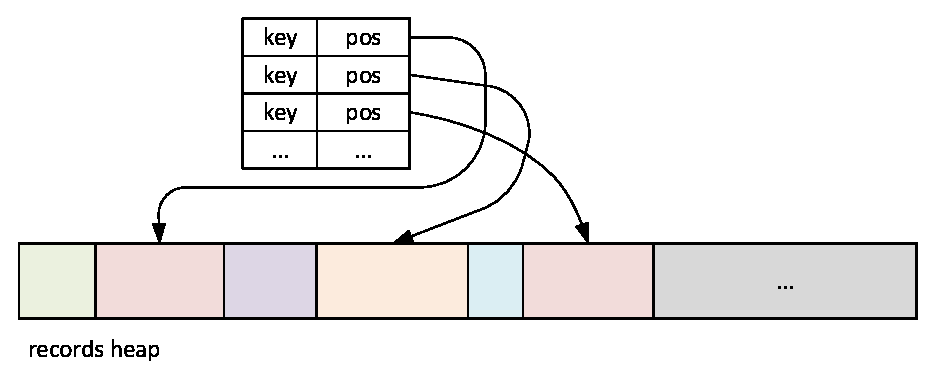
\includegraphics[width=0.8\linewidth]{handout/img/3-heap.eps}
    \caption{数组索引}\label{fig:3-heap}
\end{figure}

\begin{exercise}
    用数组来表示索引函数$f(x)$，有没有其它函数表示方案？
\end{exercise}

\subsection{稀疏索引与密集索引}

\figurename\ref{fig:3-heap}中每条记录在索引中都有一个对应的索引项，这个索引项记录了记录的key和记录的位置，这种索引称为密集索引。密集索引由于对每个记录都有索引项，整体尺寸比较大。索引结构会存放在磁盘上，要访问索引需要先调入内存，索引尺寸月大，访问时间也会增加，也不适合整体调入内存。

索引尺寸越小，io开销越小。同时考虑到并不总是要访问所有记录，所以只需要将部分索引项调入内存即可。因此，将\figurename\ref{fig:3-heap}分级，高层索引指向低层索引，低层索引指向记录，如\figurename\ref{fig:3-sparse}所示。高层索引称为稀疏索引，底层索引按需调入内存。

\begin{figure}[H]
    \centering
    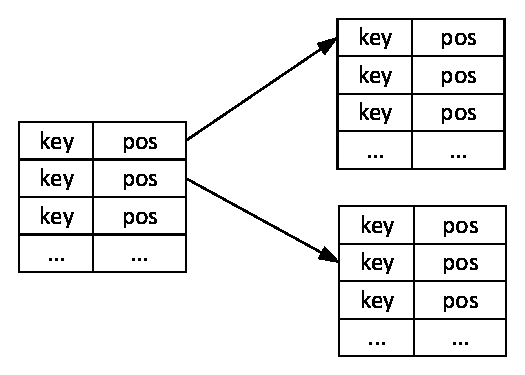
\includegraphics[width=0.5\linewidth]{handout/img/3-sparse.eps}
    \caption{稀疏索引}\label{fig:3-sparse}
\end{figure}

在\figurename\ref{fig:3-sparse}中，高层索引表项仍然是$(key, pos)$，与底层索引相同。实际上高层索引的key表示一个范围，在本文中都假设这个范围是左闭右开的区间$[key_{min}, key_{max})$。

\begin{exercise}
    分级索引下，$[key_{min}$和$key_{max})$对应于什么？最后一个索引项呢？
\end{exercise}

\begin{figure}[H]
    \centering
    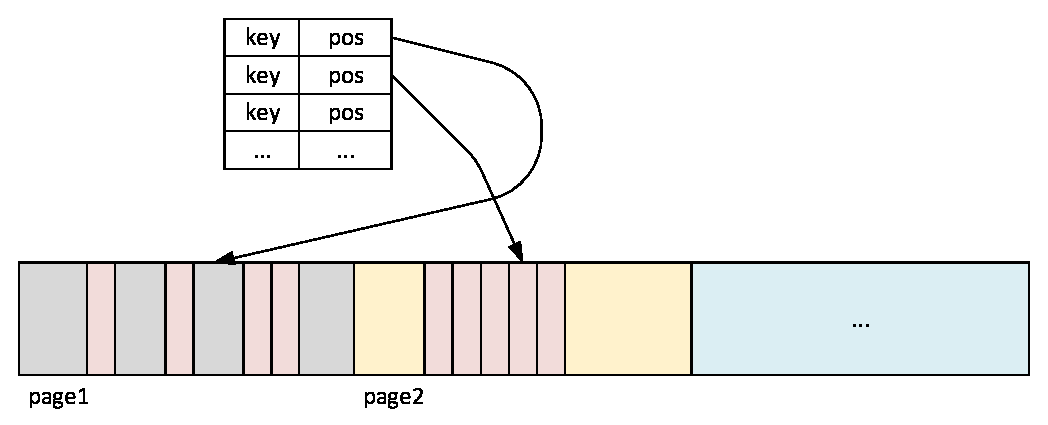
\includegraphics[width=0.8\linewidth]{handout/img/3-clustered.eps}
    \caption{聚集索引}\label{fig:3-clustered}
\end{figure}

\subsection{聚集存储与聚集索引}

\figurename\ref{fig:3-heap}中，底层存储模型为堆模型，如果采用上一章的分页模型，将key临近的记录放在临近的页面上，页面之间用指针连接起来，形成一个链表，页面的存储组织为聚集存储。考查聚集存储上的索引，key相近的记录会放在同一张页面上，页面实际上对应于一个连续的范围，因此聚集存储的索引称为聚集索引，聚集索引天然就是稀疏索引。

\begin{exercise}
    聚集存储的页面对应的范围一般不会相交，有没有相交的情况？
\end{exercise}
\begin{exercise}
    聚集存储中，两个页面临近，是指在位置上相邻吗？
\end{exercise}

实际系统中，不论是堆模型还是分页存储，都有一个问题，就是记录的位置会发生变化。如果记录的位置发生变化，索引就会失效。前述的数组方案只能用于记录位置不发生变化的情况。

\subsection{主索引与辅助索引}

主键的索引称为主索引，主索引的key是唯一的，每个记录都有一个主索引项。辅助索引的key可以重复，每个记录可以有多个辅助索引项。

\begin{figure}[H]
    \centering
    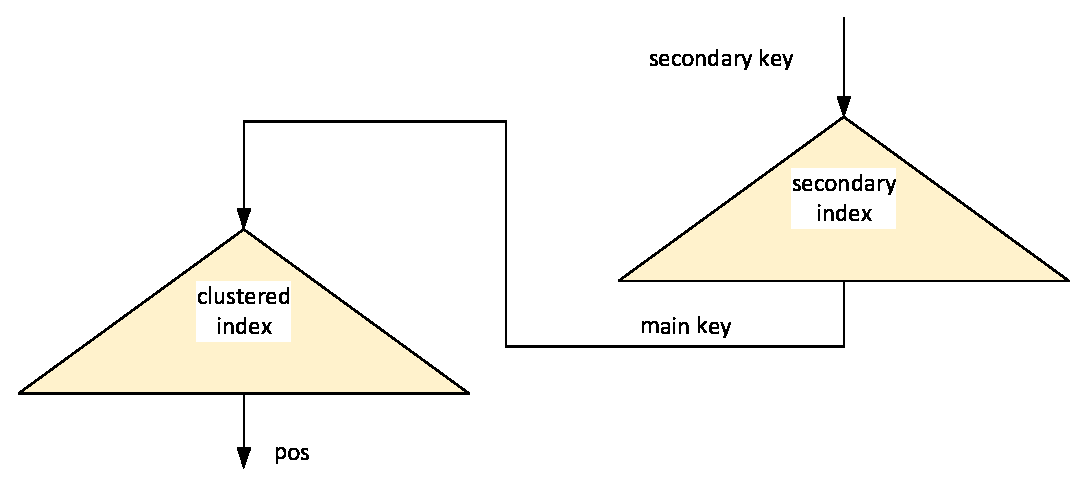
\includegraphics[width=0.8\linewidth]{handout/img/3-secondary.eps}
    \caption{聚集存储下的辅助索引}\label{fig:3-secondary}
\end{figure}

在聚集存储下，主索引是聚集存储，聚集索引给出rid一般是页面id。此时，辅助索引要检索记录的位置，需要先检索主索引，再根据主索引的结果检索记录，如\figurename\ref{fig:3-secondary}所示。

rid是一个重要概念，是记录id的简称，也可以称为rowid。聚集存储的rid一般是页面id，页面会根据key在页面的slots上确定记录在页面的偏移量。而在非聚集存储中，rid是pageid+slotid，slotid表示记录在slots数组上的下标。rid在不同系统上的称呼不同，PostgreSQL称为ctid，Oracle中称为rowid，但Oracle的rowid还会含文件号等信息。

btree里的指针实际上就是rid。

\section{btree}

索引本质上是一个搜索结构问题，在数据结构课程里有大把的搜索结构，如avl树、rbtree、hash表等。最终是btree在数据库系统中得到了广泛的应用，主要原因是btree更适合于磁盘存储。磁盘的访问单位是扇区，扇区在文件系统里组织为block，每次访问都以block为单位，btree天然适合这种访问方式。

\begin{figure}[H]
    \centering
    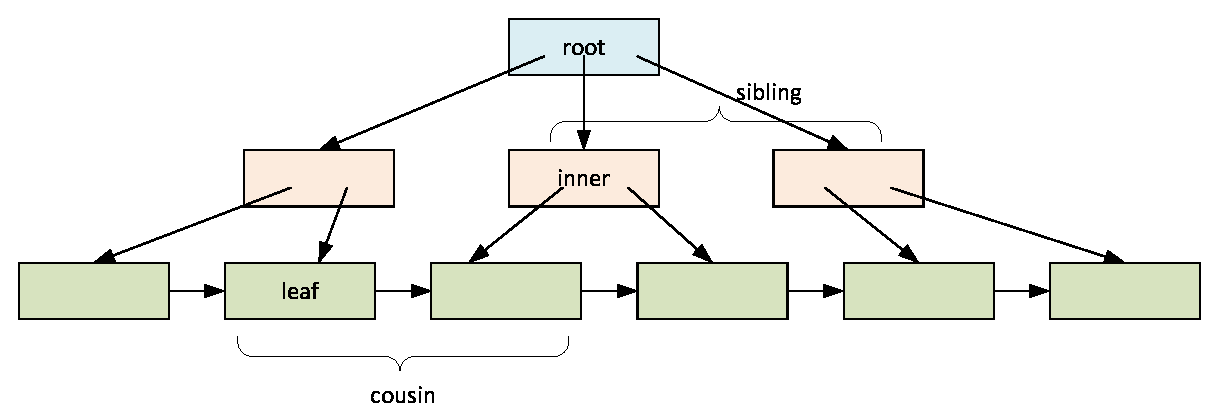
\includegraphics[width=\linewidth]{handout/img/3-btree.eps}
    \caption{btree结构}\label{fig:3-btree}
\end{figure}

btree是一种平衡多叉树，如\figurename\ref{fig:3-btree}所示，由根节点、内部节点和叶子节点构成。所有节点大小相同，在实现中，一般选择上一章的页面大小。同一个内部节点或者根节点的相邻子节点称为兄弟节点sibling，如果两个节点的父节点是兄弟节点，这两个节点称为堂兄节点cousin。

btree根节点和内部节点中，只包含key和指向子节点的指针，叶子节点包含key和指向记录的指针。并且，叶子节点之间形成一个单链表。

\begin{figure}[H]
    \centering
    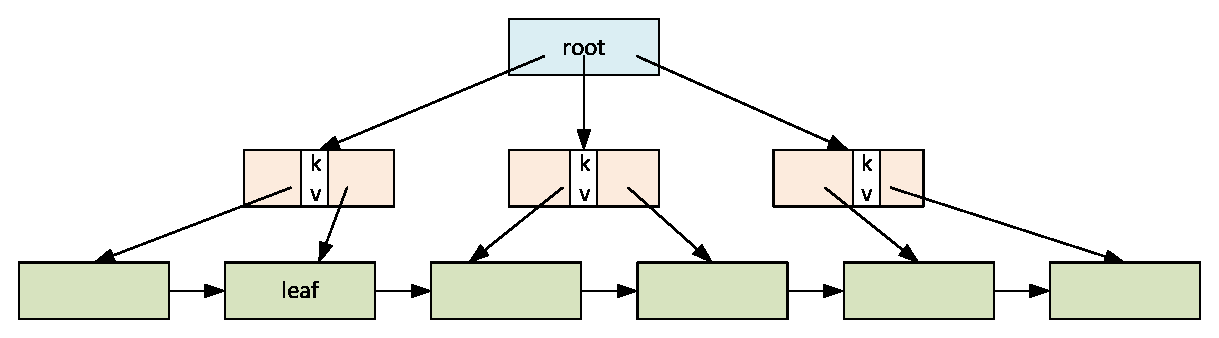
\includegraphics[width=\linewidth]{handout/img/3-btree2.eps}
    \caption{btree内部节点有kv}\label{fig:3-btree2}
\end{figure}
\begin{figure}[H]
    \centering
    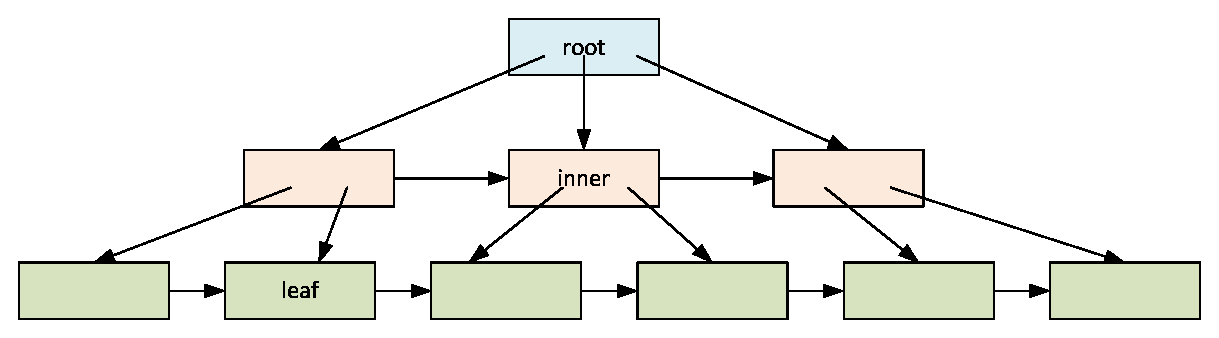
\includegraphics[width=\linewidth]{handout/img/3-bxtree.eps}
    \caption{b*tree内部节点有后继}\label{fig:3-bxtree}
\end{figure}

\subsubsection*{btree/b+tree/b*tree}

最早提出的btree虽然形如\figurename\ref{fig:3-btree}的结构，btree但叶子节点和内部节点上存储的是key+value+pos指针。本讲义中，btree实际指的是b+tree。b+tree与b*tree之间有细微区别，在b*tree中，内部节点之间也形成一个单链表。

b+tree的好处是，叶子节点、内部节点和根节点的结构完全相同，现代数据库中普遍采用b+tree作为索引。再次强调，本讲义中的btree是b+tree，而非最原始的btree。

\subsection{btree原理}

btree的叶子节点内部存储了key和pos指针，pos指针指向记录的位置，其中包括$n$个记录和$n$个记录的指针，同时还有一个指向下一个叶子节点的后继指针，如\figurename\ref{fig:3-leaf}所示。

\begin{figure}[H]
    \centering
    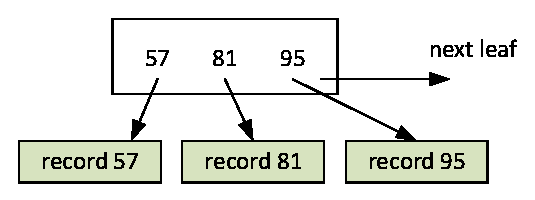
\includegraphics[width=0.5\linewidth]{handout/img/3-leaf.eps}
    \caption{btree叶子节点}\label{fig:3-leaf}
\end{figure}
\begin{figure}[H]
    \centering
    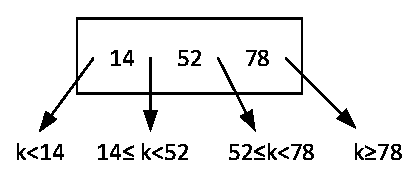
\includegraphics[width=0.4\linewidth]{handout/img/3-inner.eps}
    \caption{btree内部节点}\label{fig:3-inner}
\end{figure}

btree内部节点和根节点如\figurename\ref{fig:3-inner}所示，内部节点包含$n$个key和$n+1$个指向子节点的指针。在内部节点中，位于一个key左侧的指针表示小于这个key，位于key右侧的指针表示大于等于这个key。每个指针指向的是一颗子树，子树位于这个指针的key范围内。

\begin{figure}[H]
    \centering
    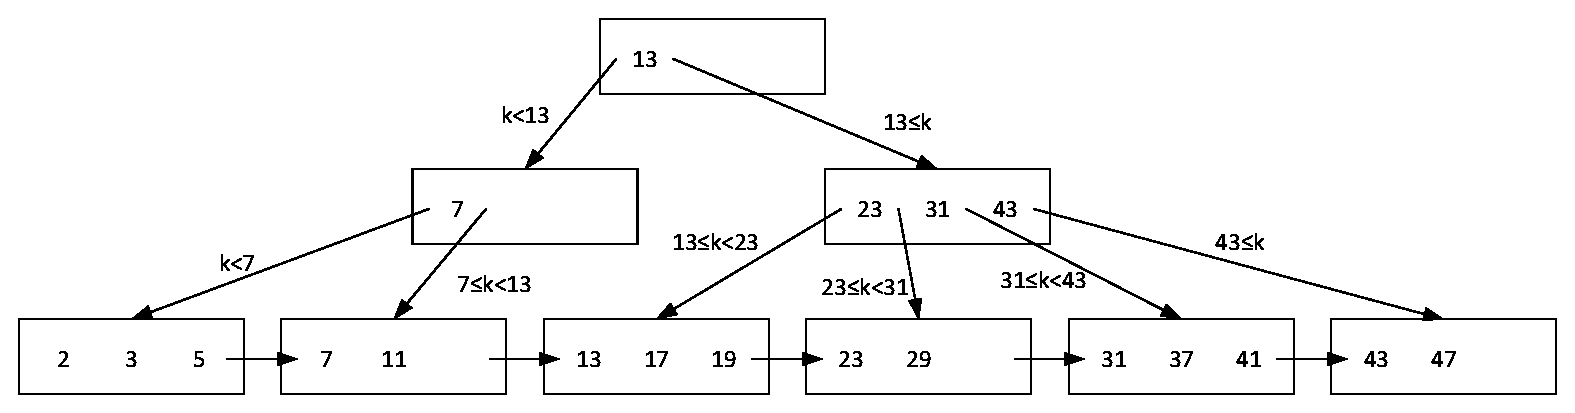
\includegraphics[width=\linewidth]{handout/img/3-btree3.eps}
    \caption{一颗完整的btree树}\label{fig:3-btree3}
\end{figure}

\figurename\ref{fig:3-btree3}是一颗完整的btree树，观察这颗树：
\begin{itemize}
    \item 观察叶子节点，除最左侧和最右侧节点外，所有叶子节点的范围是左闭右开的区间。
    \item 最左侧叶子节点是一个右开区间，最右侧叶子节点是一个左闭区间。
    \item 同理，每层中间节点的性质与叶子节点类似。
    \item 内部节点最左侧指针指向的范围需要父节点参与确定，除非该节点位于最左侧。
\end{itemize}

btree是平衡多叉树，所谓平衡是指节点的分布平衡，所有叶子节点都在同一层内。内部节点、叶子节点都要求容量过半，允许根节点容量低于一半。当key变长时，节点内包含的key和指针数目是变化的。很多教材都会采用固定长度的key来讲解btree，但要注意节点容量是变化的，或者说容量不是key的个数，而是占用节点存储尺寸。

\subsubsection*{查找}

在btree查找一个记录，很直观。从根节点开始，在根节点和内部节点上根据key确定要访问的子树，沿着子树下降，直到叶子节点。在叶子节点上，根据key确定要访问的记录。

在节点内部，使用二分搜索查找子树或者记录，查找的层数是树高，整体的时间复杂度是$O(\log n)$。

\begin{exercise}
    btree的性能一定比rbtree好吗？
\end{exercise}

实际系统中，可能在叶子节点上没有对应的记录，可能要返回小于该key的最大记录位置。并且，考虑到在插入和删除记录，需要使用查找操作来确定记录的位置，查找应该返回从根到叶子节点的整条搜索路径。

\begin{exercise}
    在\figurename\ref{fig:3-btree3}中，查找key为40的记录。
\end{exercise}

\subsubsection*{范围查找}

btree支持范围查找，这在数据库中是非常重要的操作。范围查找的方式是，先确定左边界，然后从左边界开始遍历，直到遍历到右边界。

\begin{example}
    假设执行如下SQL查询：
\begin{lstlisting}[style=verbose]
    SELECT * FROM R WHERE R.k > 40;
    SELECT * FROM R WHERE R.k >= 10 AND R.k <= 25;
\end{lstlisting}
第1条查询语句，从根节点开始，递归下降到叶子节点，找到41，然后向后枚举所有记录，过程如\figurename\ref{fig:3-lookup}所示。
\begin{figure}[H]
    \centering
    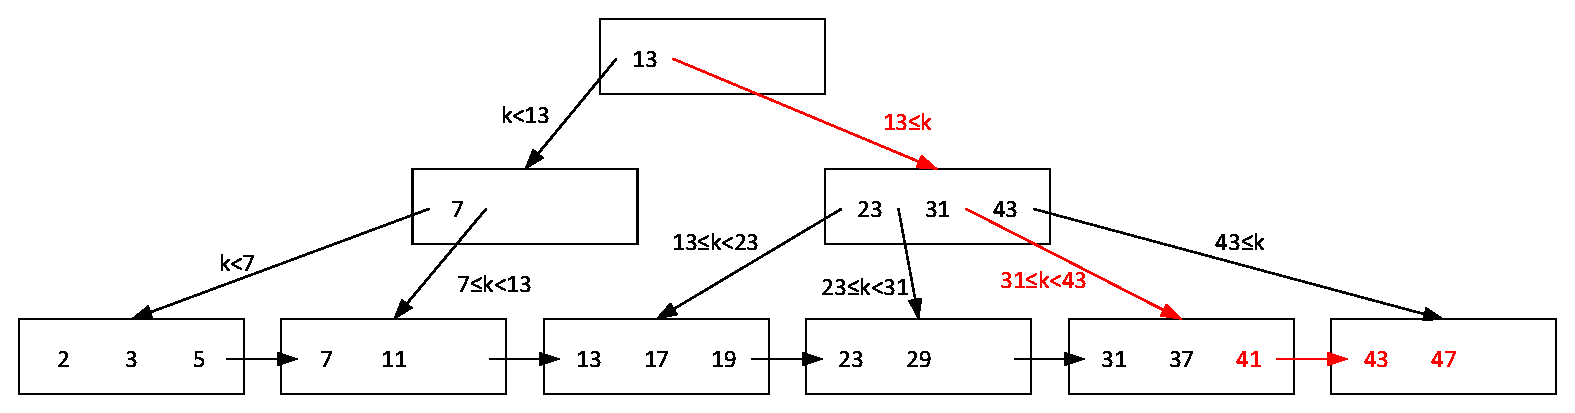
\includegraphics[width=\linewidth]{handout/img/3-lookup.eps}
    \caption{查找40后的记录}\label{fig:3-lookup}
\end{figure}
\end{example}

\begin{exercise}
    为什么btree的范围查找不需要确定右边界？
\end{exercise}
\begin{exercise}
    在\figurename\ref{fig:3-btree3}中，查找key为10到25的记录。
\end{exercise}

\subsubsection*{插入}

在btree中插入一条记录，需要先查找记录的位置，然后在叶子节点上插入记录。如果插入后导致节点容量超过上限，需要进行分裂。节点分裂，意味着多出了一个指针，需要在父节点上新增这个指针。这个过程是从叶子节点向根递归，直到根节点，如果根节点的容量不够，还需对根节点分裂，此时意味着树的高度增加了一层。

节点分裂的标准是，节点的容量超过上限时，分裂成两个节点，每个节点容量减半。实际系统中，由于key可能变长，容量是指节点的存储尺寸，而不是key的个数。并且，由于key变长，这种分裂可能并不一定会很均匀，但实际应用中问题不大。

\begin{exercise}
    证明key变长时，btree仍然是平衡的。
\end{exercise}

\begin{example}
    在\figurename\ref{fig:3-btree3}中，插入key为40的记录。首先在叶子节点上插入，叶子接点分裂如\figurename\ref{fig:3-insert1}所示：
\begin{figure}[H]
    \centering
    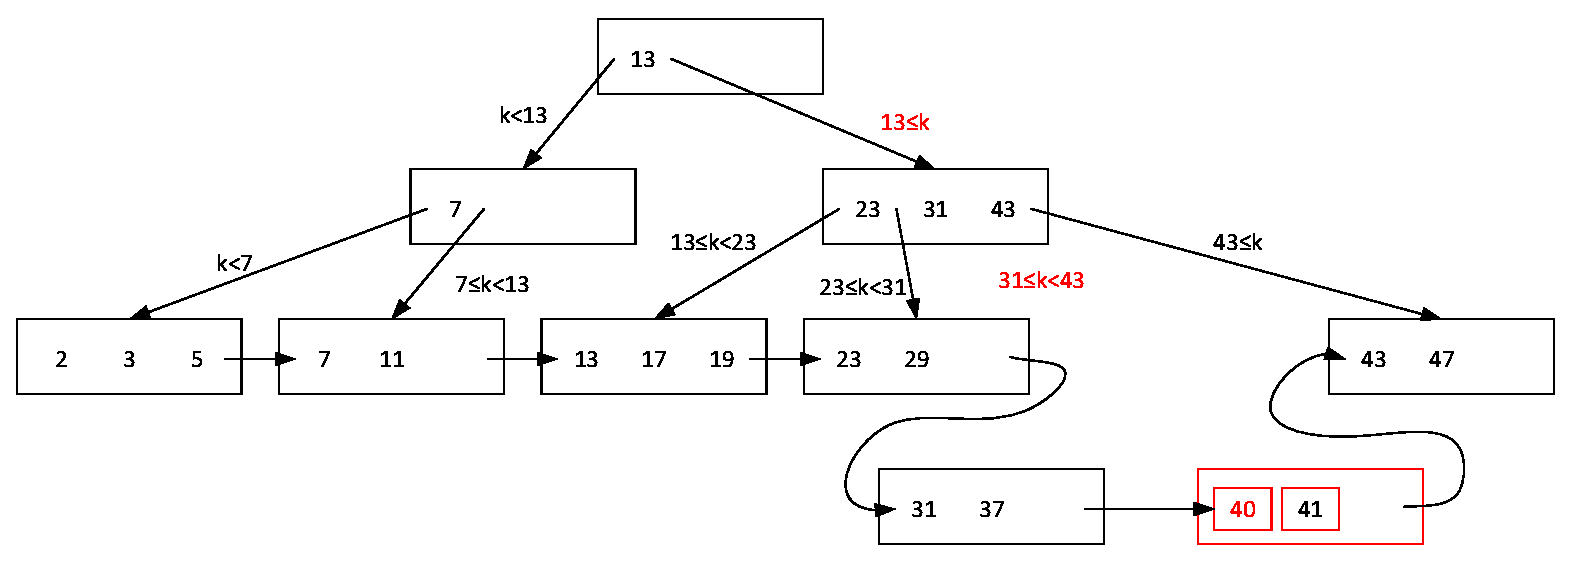
\includegraphics[width=\linewidth]{handout/img/3-insert1.eps}
    \caption{叶子节点分裂}\label{fig:3-insert1}
\end{figure}
新增叶子节点放在原叶子节点之后，然后需要递归向上插入新的指针。新增指针指向新节点最左侧的key，对应于\figurename\ref{fig:3-insert1}的40。这个40的key要在父节点上插入，如果父节点容量也超过上限，需要继续分裂。
\begin{figure}[H]
    \centering
    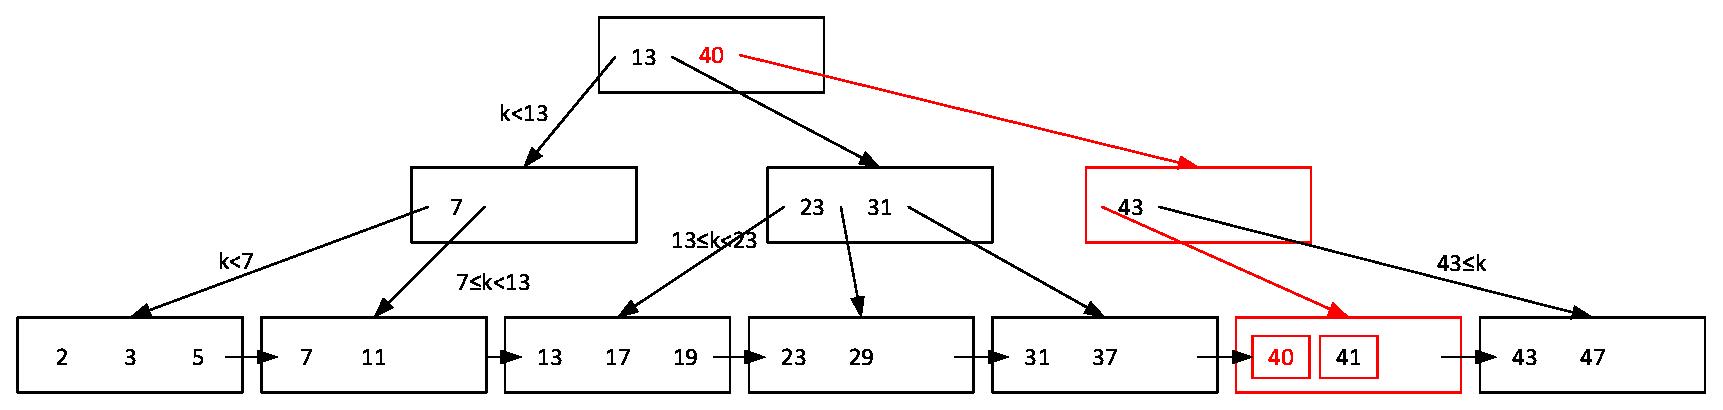
\includegraphics[width=\linewidth]{handout/img/3-insert2.eps}
    \caption{内部节点分裂}\label{fig:3-insert2}
\end{figure}
但是内部节点分裂不同于叶子节点分裂，新的内部节点需要将最左侧的key上移到父节点上，对应于\figurename\ref{fig:3-insert2}中的根节点。为什么不同？设想一下，4个key，5个指针，按照key分裂为2+2形式，2个节点会有6个指针。新内部节点上移，相当于带走了一个指针。
\end{example}

\begin{exercise}
    新增叶子节点为什么要放在右侧？同理，新增内部节点也需要放在右侧？
\end{exercise}

\subsubsection*{删除}

删除一条记录，需要先查找记录的位置，然后在叶子节点上删除记录。如果删除后导致节点容量低于下限，需要向临近的兄弟节点借，如果兄弟节点出借后，也低于下限，就需要将两个兄弟节点合并。

\begin{example}
    在\figurename\ref{fig:3-insert2}中，删除key为7的记录。删除7对应的记录后，叶子节点容量不够，需要向兄弟节点借记录。
\begin{figure}[H]
    \centering
    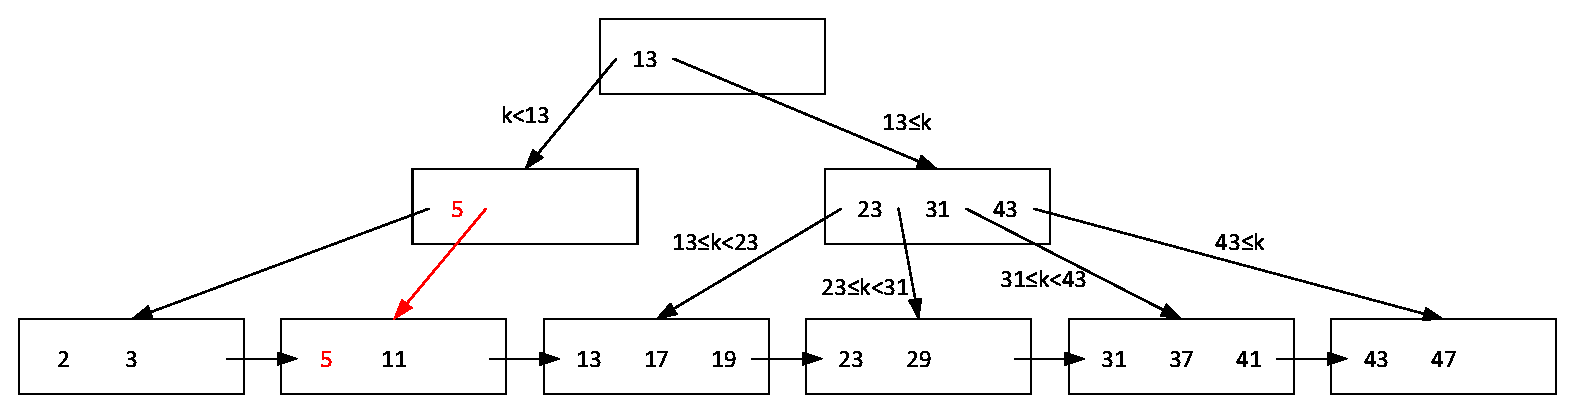
\includegraphics[width=\linewidth]{handout/img/3-delete.eps}
    \caption{删除7后的记录}\label{fig:3-delete}
\end{figure}
由于借到了5的记录，叶子节点的最左key发生变化，父节点的key也需要相应变化。
\end{example}

删除记录，导致叶子节点容量不够，向兄弟节点借记录。兄弟节点有两个，一个是左侧，一个是右侧。如果向左侧兄弟借，会改变节点的最左侧key，该叶子节点的指针对应的key也需要变化。借右侧兄弟节点，需要调整指向右侧节点的指针和key。

\begin{example}
    在\figurename\ref{fig:3-delete}中，删除key为11的记录。删除11对应的记录后，叶子节点容量不够，需要向兄弟节点借记录，如\figurename\ref{fig:3-delete2}所示。
\begin{figure}[H]
    \centering
    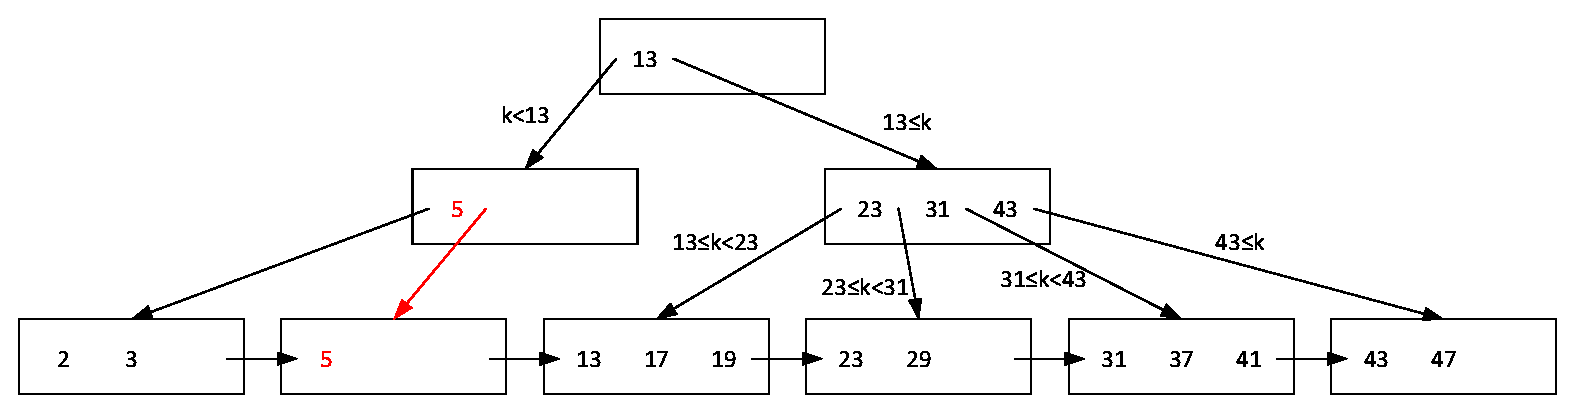
\includegraphics[width=\linewidth]{handout/img/3-delete2.eps}
    \caption{删除11后的记录-1}\label{fig:3-delete2}
\end{figure}
由于右侧没有兄弟节点，只能向左侧兄弟借记录，但左侧兄弟节点仍然不够，因此只能合并。合并后，删除该叶子节点，父节点中，指向该节点的指针和key也需要删除，对应于\figurename\ref{fig:3-delete3}所示：
\begin{figure}[H]
    \centering
    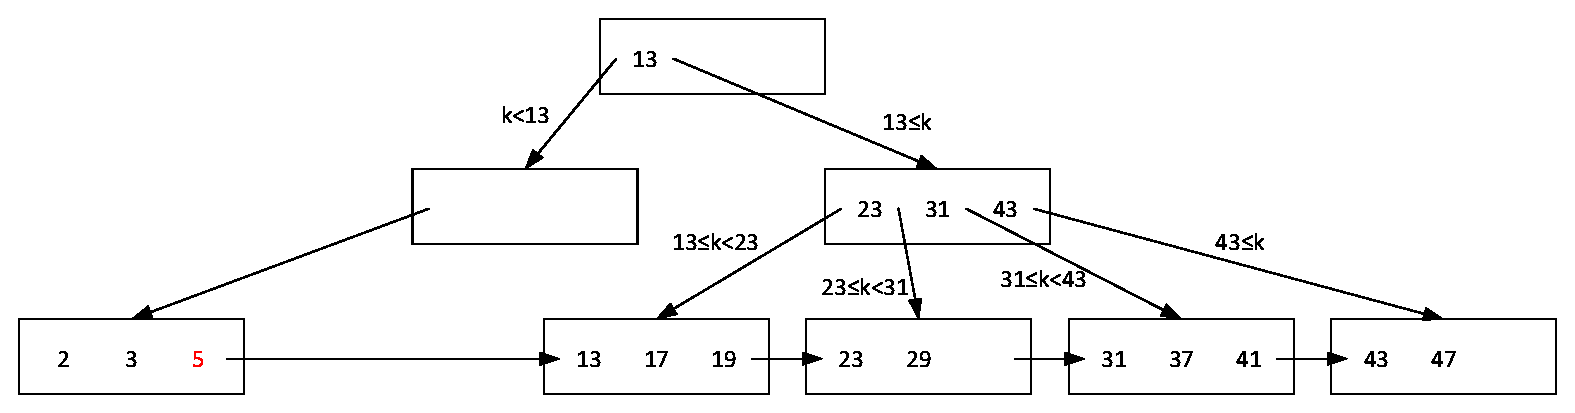
\includegraphics[width=\linewidth]{handout/img/3-delete3.eps}
    \caption{删除11后的记录-2}\label{fig:3-delete3}
\end{figure}
\begin{figure}[H]
    \centering
    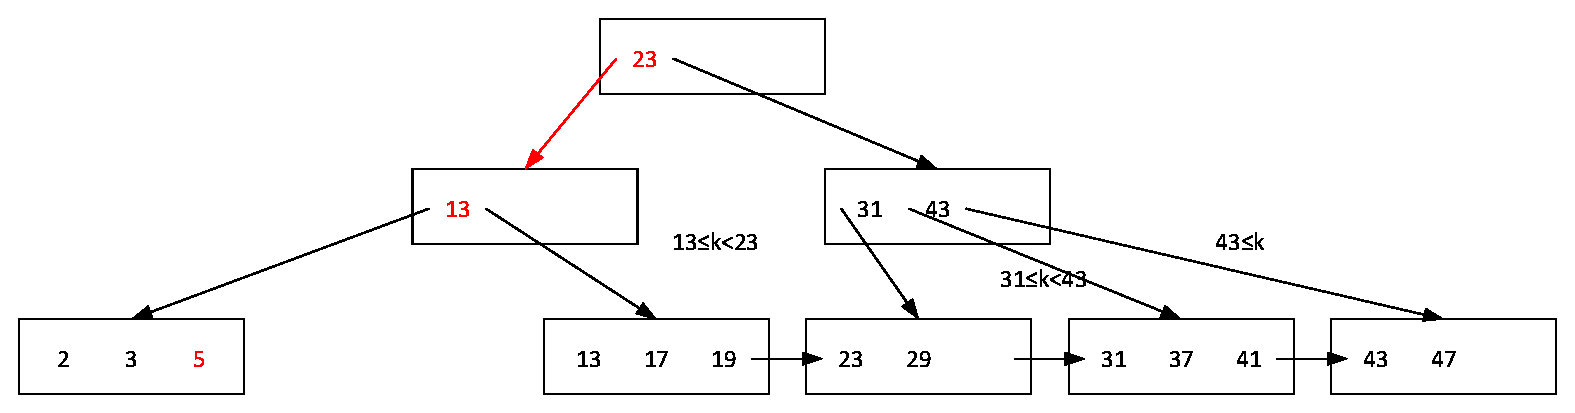
\includegraphics[width=\linewidth]{handout/img/3-delete4.eps}
    \caption{删除11后的记录-3}\label{fig:3-delete4}
\end{figure}
接下来考虑内部节点的情况。内部节点删除key和指针后，可能导致节点容量低于下限，需要向临近的兄弟节点借记录。如果借到的记录也低于下限，就需要将两个兄弟节点合并。内部节点借兄弟节点，也比较麻烦，需要同时调整父节点和兄弟节点，对应于\figurename\ref{fig:3-delete4}所示。
\end{example}

出借记录的情况比较复杂，这里需要总结一下。
\begin{itemize}
    \item leaf：叶子节点向兄弟节点借记录。确定截断位置，将内部节点的key改为截断位置后面的key。
\begin{figure}[H]
    \centering
    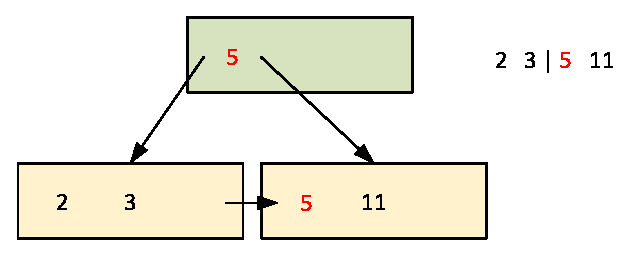
\includegraphics[width=0.5\linewidth]{handout/img/3-leaf-borrow.eps}
    \caption{叶子节点borrow}\label{fig:3-leaf-borrow}
\end{figure}
    \item inner：内部节点向兄弟节点借记录。两个内部节点一定是由某个key分隔，出借要将父节点的key考虑在内，如\figurename\ref{fig:3-inner-borrow}所示。确定截断位置，将父节点的key改为截断位置后面的key。
\begin{figure}[H]
    \centering
    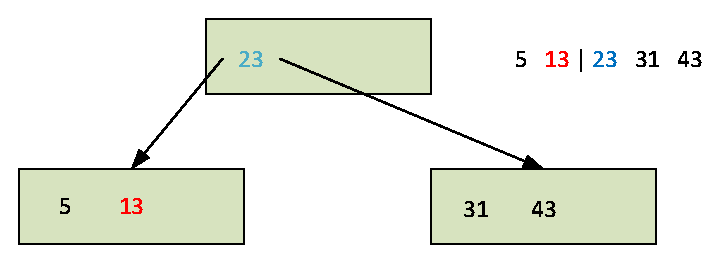
\includegraphics[width=0.5\linewidth]{handout/img/3-inner-borrow.eps}
    \caption{内部节点borrow}\label{fig:3-inner-borrow}
\end{figure}
\end{itemize}

\subsection{btree优化}

btree是数据库广泛采用的索引结构，对它的研究比较透彻，优化角度也比较多。

\begin{figure}[H]
    \centering
    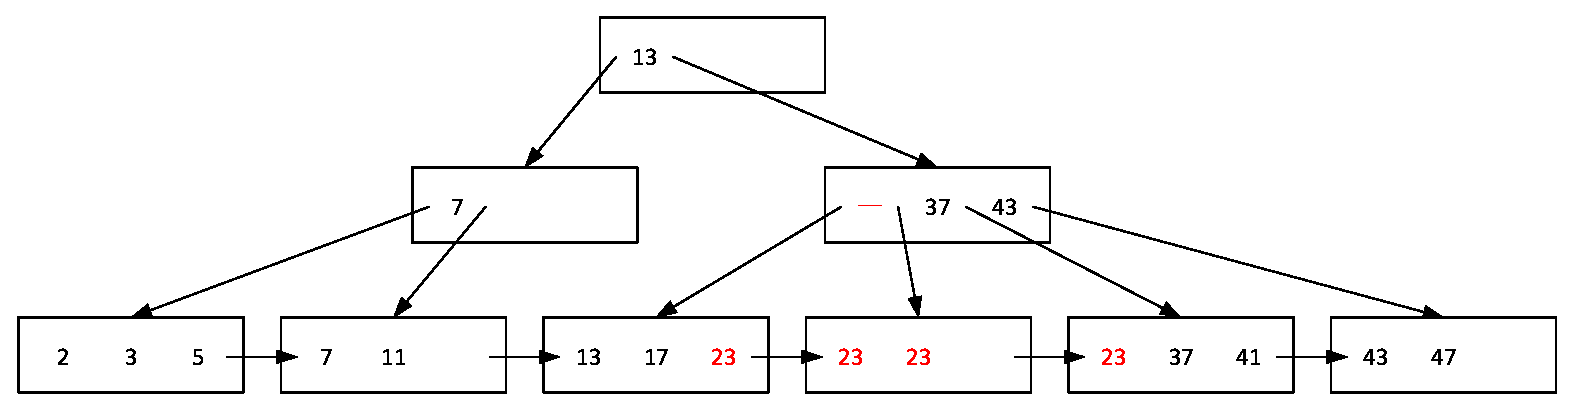
\includegraphics[width=\linewidth]{handout/img/3-duplicate.eps}
    \caption{重复键}\label{fig:3-duplicate}
\end{figure}

\subsubsection*{重复键}

主索引的key都是唯一的，但是辅助索引的key可以重复。重复键的处理方案可以有很多种，一种是直接将重复键的记录指针罗列在叶子节点中，对应于\figurename\ref{fig:3-duplicate}所示。这种方案的主要问题是，重复键过多，可能占用整个叶子节点，这会影响到内部节点的key如何处理。在\figurename\ref{fig:3-duplicate}中，23对应的key值在内部节点中用—来表示，意思是这个key值为null。当key值为null时，意思是整个叶子节点重复前面的key值。

\begin{exercise}
    如何表达key为—？或者说如何在数据库内部表达null？
\end{exercise}

另一种解法是利用记录格式来处理。重复键只能出现在辅助索引中，并且只能出现在辅助索引的叶子节点上，此时可以将这些指向重复键的记录指针顺序的排列在一条记录里。

\begin{figure}[H]
    \centering
    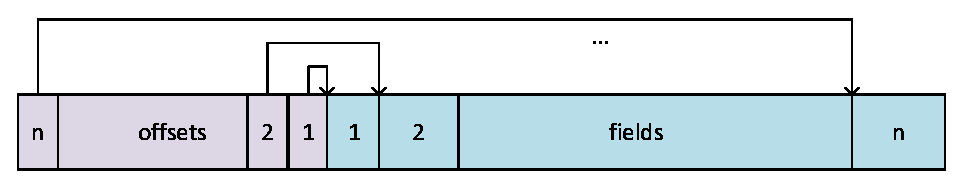
\includegraphics[width=0.8\linewidth]{handout/img/3-duplicate2.eps}
    \caption{将所有重复键的记录顺序罗列在一条记录}\label{fig:3-duplicate2}
\end{figure}

\subsubsection*{性能}

btree总是从根节点开始搜索，整个路径长度为树的高度。每次加载根节点都会产生一次io，io操作非常慢，一个很自然的方案是将根节点时刻缓冲起来。这样每次搜索就节省一次io，算总账的时候会节省很多io。

这个优化方案还可以更贪婪，将btree的高层都缓冲起来。这样每次搜索就节省更多的io。

\subsubsection*{页面格式}

btree的页面大小是上一章的页面大小，页面结构也与上一章相同。假设btree的节点要保存$n$个key，$n+1$个指针，一般是将$<key, ptr>$处理为一条记录，ptr是key右侧指针。页面尾部按照上一章介绍的slots数组维护。内部节点和根节点，最左侧的ptr使用页面头部的next指针存储。

\subsubsection*{前缀压缩}

由于btree中key是有序的，非常适合做前缀压缩。前缀压缩技术可以参考leveldb\cite{GitHubgo38:online}，在上一章也有过介绍。可以将整个page看成是leveldb的datablock，多个kv构成一组，取第1个key的前缀作为压缩前缀，后续key只需要存储与压缩前缀的差异即可。在page的尾部设置slots数组，维护各组的索引。

应用前缀压缩的前提是key要看成二进制字符串，leveldb中简单地用memcmp比较key。在关系数据库中，许多系统先经过collation校对后，再按照二进制字符串比较。

\subsubsection*{top-down策略}

节点分裂从叶子节点开始，向上递归分裂，直到根节点。这个过程与搜索过程相反，在latch节点时，容易出现死锁。可以先计算需要分裂的高度，然后从上向下分裂，分裂完毕后，再插入新记录。

同理，在删除记录时，也应该先计算需要合并的高度，然后从下向上合并或者出借。

\subsubsection*{延迟合并}

删除记录，会导致记录出现在不同的叶子节点或者内部节点，为保证搜索路径的正确性，必须使用拍它的latch，会阻塞其他线程的搜索。

有些系统假设表总是膨胀的，在删除记录后不会立即合并节点，也不主动向兄弟节点借记录。——这种方案可能会出现空节点。

\subsection{范围锁}

在后文介绍事务并发时，会使用范围锁来解决幻读问题，这里简单描述一下幻读问题。

假设系统运行在Read Commited, RC隔离级别及以下。有一张表phantom\_test，它有一个主键列id。两个事务a和b，交替执行以下操作：
\begin{lstlisting}[style=verbose]
-- 事务a第一次查询
BEGIN;
SELECT * FROM phantom_test WHERE id > 3 AND id < 8 FOR UPDATE;
-- 结果: id=5 (Bob)

-- 事务b
BEGIN;
INSERT INTO phantom_test VALUES (6, 'David');
COMMIT;

-- 事务a第二次查询（同一事务内）
SELECT * FROM phantom_test WHERE id > 3 AND id < 8 FOR UPDATE;
-- 结果: id=5 (Bob), id=6 (David)
COMMIT;
\end{lstlisting}

在上面的例子中，事务a第一次查询id大于3小于8的记录，结果只有id为5的记录。然后事务b插入了id为6的记录。事务a第二次查询id大于3小于8的记录，结果有id为5和6的记录。这就发生了幻读问题。

在后文的锁方案中，要杜绝幻读的发生，需要使用范围锁，即对查询的范围加锁，防止其他事务在这个范围插入记录。

\subsubsection*{区间范围}

WHERE语句使用的条件称为谓词predicate，就是限定词，谓词逻辑中使用限定词为$\forall, \exists$，SQL里使用的限定词要更复杂一些。谓词在最后被处理为一个或多个范围，这些范围的开闭有四种情况，如\figurename\ref{fig:3-gap}所示。

\begin{itemize}
    \item $[a, b]$：闭区间，包含a和b。
    \item $(a, b)$：开区间，不包含a和b。
    \item $[a, b)$：闭区间，包含a不包含b。
    \item $(a, b]$：开区间，不包含a包含b。
\end{itemize}

\begin{figure}[H]
    \centering
    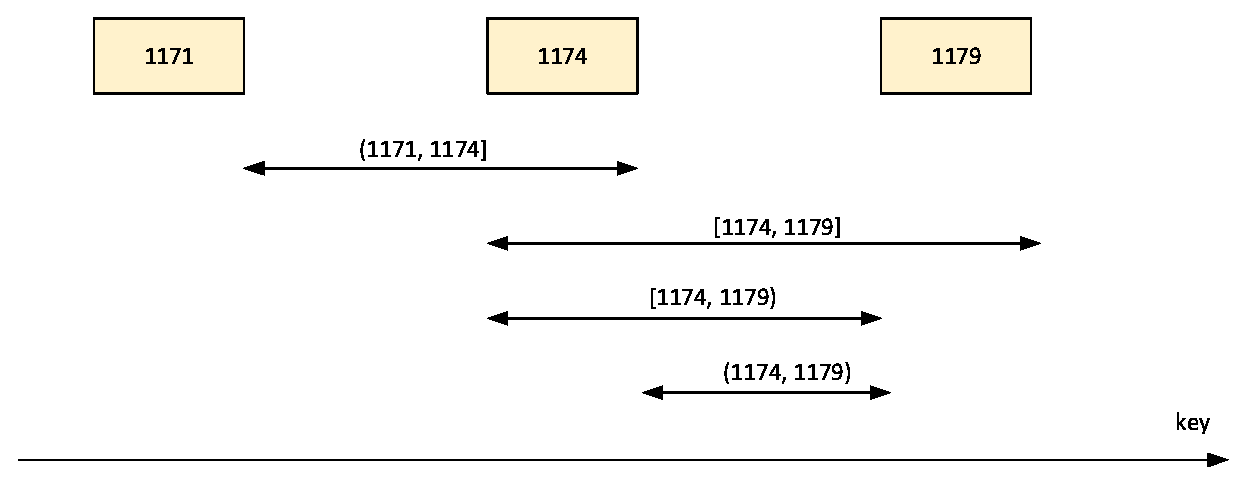
\includegraphics[width=0.8\linewidth]{handout/img/3-gap.eps}
    \caption{各种区间范围}\label{fig:3-gap}
\end{figure}

\subsubsection*{锁表}

在下一章会更详细介绍锁表，锁表是一个内存结构，一般用hash表构建。给定一个key，会先在锁表中查找是否有对应的锁。如果没有，就创建一个新的锁。如果有，则返回key对应的锁。\figurename\ref{fig:3-locktable}的锁表是一个点锁表，还不支持范围锁，接下来要扩展这个结构支持范围锁。

\begin{figure}[H]
    \centering
    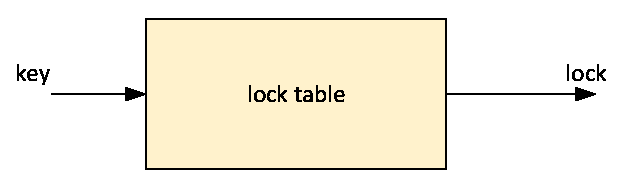
\includegraphics[width=0.6\linewidth]{handout/img/3-locktable.eps}
    \caption{锁表示意图}\label{fig:3-locktable}
\end{figure}

\subsubsection*{gap锁}

WHERE条件的谓词，可以直接处理为锁。每次想要获取锁时，先执行一下这个谓词，如果返回为true，就获取锁。但这种方案开销巨大，所有事务都必须无差别执行一遍谓词。解决方案是将这个谓词范围映射到btree的叶子节点上，在每个叶子上维持一个局部的小范围锁，如\figurename\ref{fig:3-gap2}。

每个btree叶子节点对应于一个锁管理结构，它管理叶子上的所有gap锁，包括点锁。这个管理结构以叶子节点的指针为key，注册到锁表。当搜索到叶子节点，就查找锁表获取这个结构。

\begin{figure}[H]
    \centering
    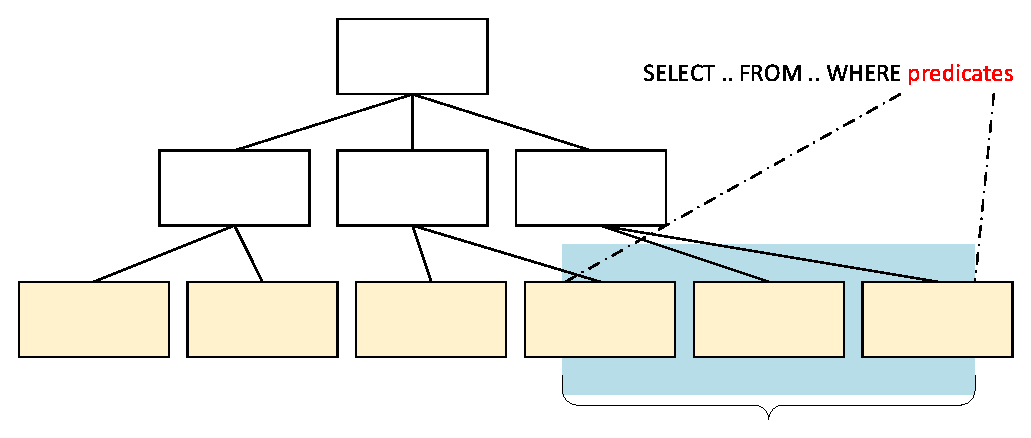
\includegraphics[width=\linewidth]{handout/img/3-gap2.eps}
    \caption{谓词映射为gap锁}\label{fig:3-gap2}
\end{figure}

\begin{exercise}
    gap锁为什么不在中间节点和内部节点上实现？
\end{exercise}

称叶子节点上的锁管理结构为leaf lock manager，它使用一个链表管理所有gap锁，需要加锁时要逐个测试这些gap锁。为了加快测试，可以将这个链表组织成一个区间树，每个区间对应一个gap锁。另外，为了判断是否加锁，使用bitmap来标记叶子上每个区间是否加锁。

\begin{figure}[H]
    \centering
    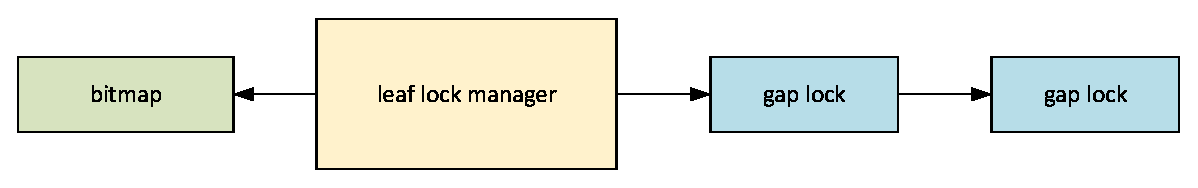
\includegraphics[width=\linewidth]{handout/img/3-leaflock.eps}
    \caption{叶子节点上的gap锁}\label{fig:3-leaflock}
\end{figure}

当使用bitmap来判断一个key是否落入某个区间时，实现上有些问题。gap锁的区间与叶子节点上的记录区间并不对齐，如\figurename\ref{fig:3-interval}所示。\figurename\ref{fig:3-leaflock}里的bitmap是用slots[]数组来标定，因此借用bitmap来判断是否加锁可能会出现误报，需要进一步使用链表来确定是否加锁。

\begin{exercise}
    为什么用slots[]数组来标定gap锁的区间？
\end{exercise}
\begin{exercise}
    如果使用gap树而非链表，是否可以省略掉bitmap？
\end{exercise}

\begin{figure}[H]
    \centering
    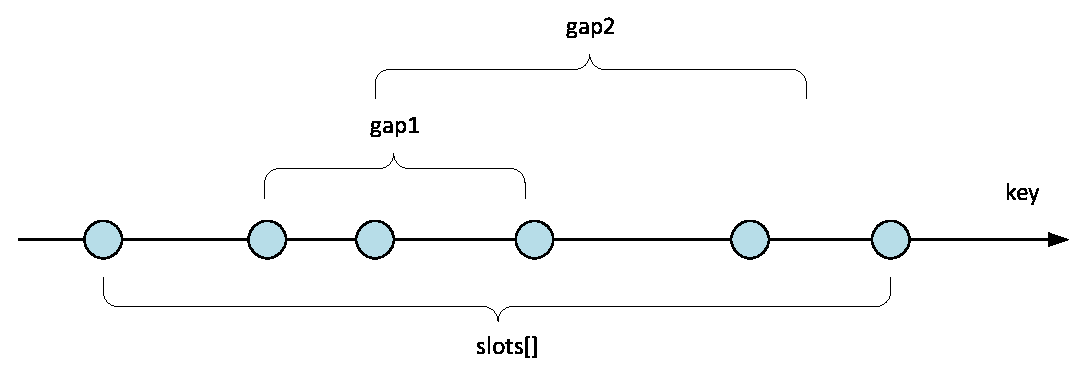
\includegraphics[width=\linewidth]{handout/img/3-interval.eps}
    \caption{gap与slots[]数组不对齐}\label{fig:3-interval}
\end{figure}

\section{skiplist}

跳表是kv存储中最常见的数据结构。kv存储一般采用append追加模型，数据写入后不再修改，这种模型与传统关系数据库中读写平衡的设计不同。kv存储的索引结构分为两部分，一是活动内存结构，二是持久化结构。活动结构用于索引未落盘的数据，参考\figurename\ref{fig:2-lsm}。持久化结构用于索引已落盘的数据，由于不会改变，就是有序数组，如\figurename\ref{fig:3-heap}。

leveldb是一个成熟的kv存储引擎，它的活动索引为跳表。之所以选择跳表，有几方面的原因：一是跳表是一写多读的lockfree结构，对多核系统支持较好。二是跳表天然支持范围查询，这在kv存储中是一个重要的功能。三是跳表的实现比较简单，容易理解和维护。四是跳表一开始就要设定容量，而在kv存储中，这不是问题。

\subsection{跳表结构}

跳表需要在内存中动态构建，它的基础数据结构是单链表，为了加快查询，它概率的在某些节点上建立多层的后向指针。

跳表结构如\figurename\ref{fig:3-skiplist}，head是一个多层的后向指针，初始化指向null，n是跳表中的节点数目。表中的节点除了存储数据外，还带有随机数目的层，每层指向同层的后继节点。这个随机层数与该节点插入时n的数目有关，当一个节点插入时，它取的层数服从均匀分布$l \sim U(1, \lfloor \log_2(n) \rfloor)$，在实现中这个$\lfloor \log_2(n) \rfloor$很容易计算，只需看n的哪个高位是1即可。

在levelDB的代码中，跳表节点表示如下。next是变长的一个原子指针数组，可以原子的方式修改指针。key是搜索键，结构中只定义了1个指针长度，需要在该节点构造时临时确定这个数组的大小。
\begin{lstlisting}[style=c++]
template<typename Key, class Comparator>
struct SkipList<Key,Comparator>::Node {
    Key const key;
    port::AtomicPointer next_[1];
};
\end{lstlisting}

\begin{figure}[H]
    \centering
    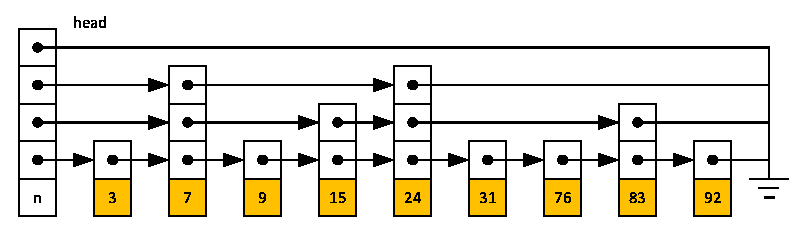
\includegraphics[width=\linewidth]{handout/img/3-skiplist.eps}
    \caption{跳表结构}\label{fig:3-skiplist}
\end{figure}

leveldb的跳表是一写多读的，只能有一个线程写入，原因是跳表是lockfree的，如果多写会丧失这些特性。leveldb采用c++实现，不支持删除操作。在leveldb实现中，节点分配使用了arena内存池，所以跳表节点没有析构函数。

\begin{exercise}
    加载一个\figurename\ref{fig:2-block}的sst文件，是否还需要构建跳表？
\end{exercise}
\begin{exercise}
    分析leveldb源码中，arena内存池是如何实现的？
\end{exercise}
\begin{exercise}
    跳表的容量如何确定？可不可以动态修改？
\end{exercise}

\subsection{功能}

跳表的搜索复杂度为$O(\log n)$，插入复杂度为$O(\log n)$，性能不弱于rbtree、btree。

\subsubsection*{查询}

跳表查询从head开始，从高层向底层迭代：1)~当碰到后继指针为null，向底层迭代；2)~如果后继节点的key比查询的键大，向下层迭代。\figurename\ref{fig:3-skiplist2}是查询9的例子。

\begin{figure}[H]
    \centering
    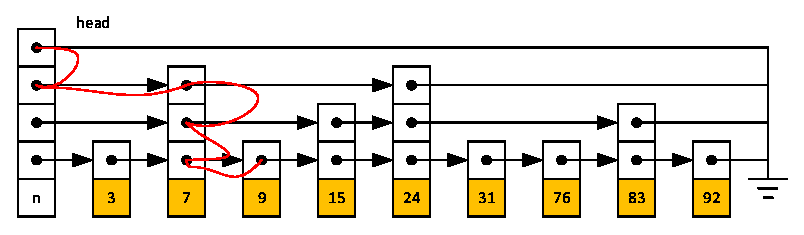
\includegraphics[width=\linewidth]{handout/img/3-skiplist2.eps}
    \caption{查询9的例子}\label{fig:3-skiplist2}
\end{figure}

在跳表上做范围查找，也是容易的，首先定位起始的节点，然后沿着最底层向后枚举即可。

\subsubsection*{插入}

在跳表上插入，首先要找到小于等于键的最大位置，然后分配节点，准备插入。由于新分配的节点可能有多层，为了将多层引入跳表，需要在定位插入位置时，保存所有层次的前驱节点。自上而下先初始化指向后继节点，然后自下而上修改前驱节点指向新增节点。

\begin{figure}[H]
    \centering
    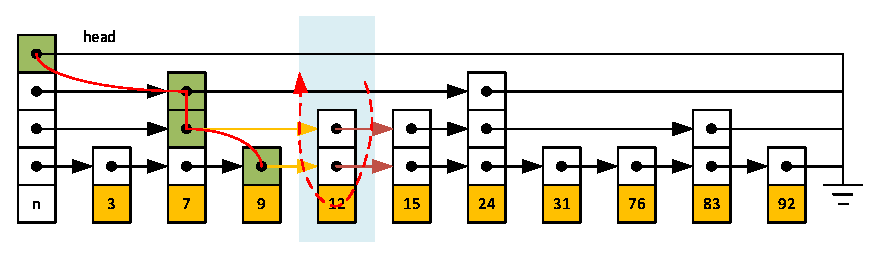
\includegraphics[width=\linewidth]{handout/img/3-skiplist3.eps}
    \caption{跳表插入}\label{fig:3-skiplist3}
\end{figure}

如\figurename\ref{fig:3-skiplist3}，要插入一个新节点12，先保存所有搜索路径。然后随机分配了一个2层的节点，自上而下先设置12节点的后继指针，然后修改前驱指针指向12。

\begin{exercise}
    跳表为什么不支持删除操作？还是leveldb里不支持？leveldb为什么不支持删除？
\end{exercise}
\begin{exercise}
    分析一下，跳表能否支持多写多读？
\end{exercise}

\section{rtree}

关系数据库的索引都是一维索引，实际的应用中存在着多维索引的需求。在诸如地理信息系统这样的应用中，数据按照二维或三维组织，这个时候就需要根据多维索引查找。

但是，多维索引的数据模型与一维索引的数据模型不同，如图\ref{fig:3-map}，地图上的图元有点、线、面的形式。点表示一个位置，线可能是一条道路，面可能是一栋大楼，线和面可以是任意形状的，例如道路可以是曲线，大楼可能是异形的。

地理信息系统GIS的数据模型与关系数据库的表不同，需要在SQL语言基础上做一些扩展，增加如下查询方式：
\begin{enumerate}
    \item 范围查询。给定任意形状的范围，搜索哪些图元在这个范围中。
    \item 邻居查询。给定一个图元，查找最近的图元。
    \item 定位查询。给定一个图元，定位包含该图元其它图元有哪些。
\end{enumerate}

空间索引是对存储在介质上的数据位置信息的描述，用来提高系统对数据获取的效率。空间索引的设计需要适应它的应用方式与图元的特性，例如电子地图需要由粗到细的刻画图元，图元的形状可能是任意的，rtree就比较合适。而在向量数据库中，由于维度很高，目标多为点且稀疏，用rtree来描述就不太合适。

\begin{figure}[H]
    \centering
    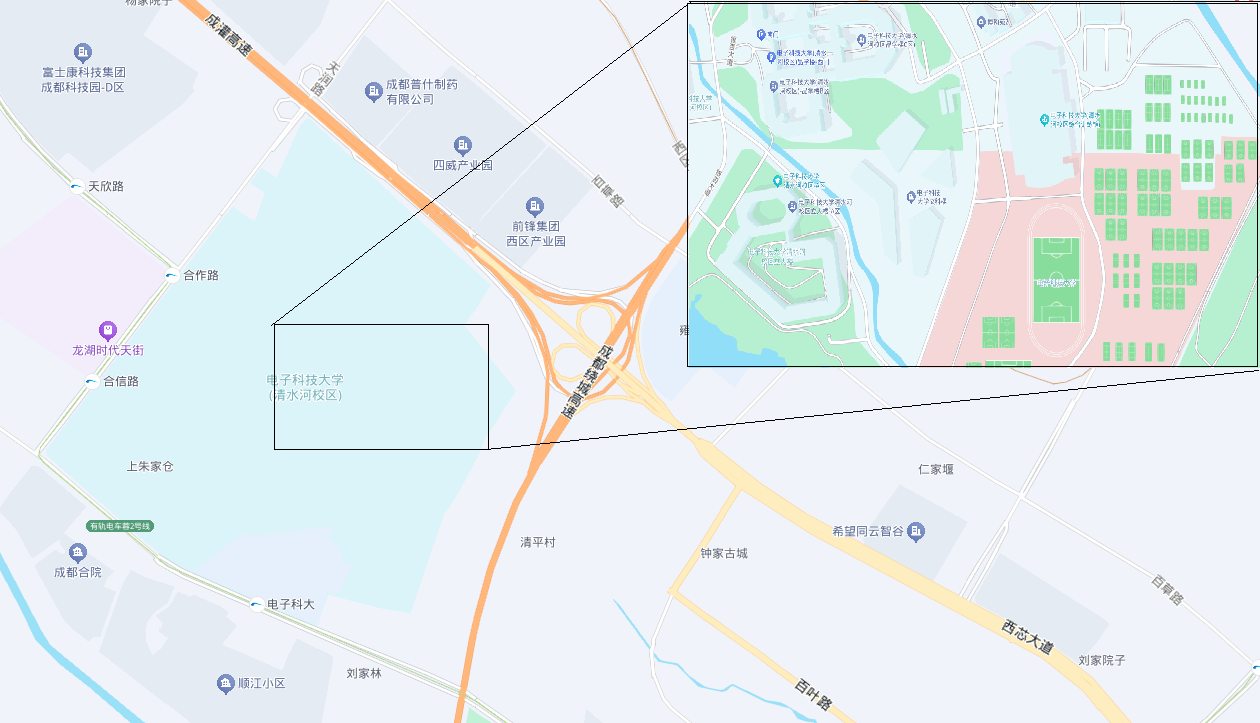
\includegraphics[width=\linewidth]{handout/img/3-map.png}
    \caption{二维地图与缩放}\label{fig:3-map}
\end{figure}

\subsection{rtree原理}

在rtree中，点、线、面使用bounding box来统一表示，如\figurename\ref{fig:3-rtree1}所示。在这个视场内，bounding box是最小的图元单位，它们之间可能彼此相交或者包含。在电子地图中，图元存放了对应的形状、坐标等信息。

\begin{figure}[H]
    \centering
    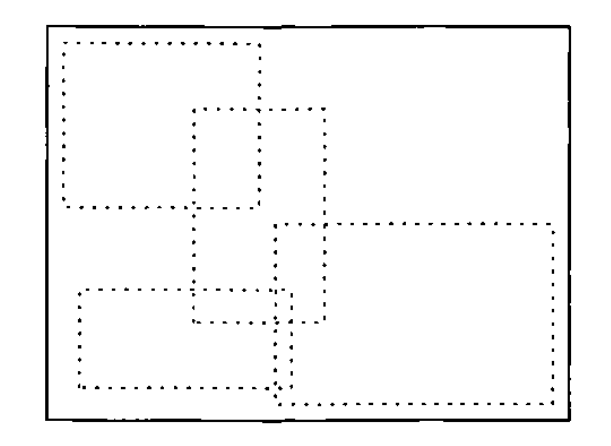
\includegraphics[width=0.6\linewidth]{handout/img/3-rtree1.png}
    \caption{bounding box示意图}\label{fig:3-rtree1}
\end{figure}

接下来需要考虑的是如何组织这些bounding box，以方便地进行范围查询。rtree的思路是在底层bounding box基础上，使用多个bounding box的并充当更高层的bounding box。通过分层的bounding box，就可以将视场分为多个区域，每个区域下会有多个图元。

\begin{figure}[H]
    \centering
    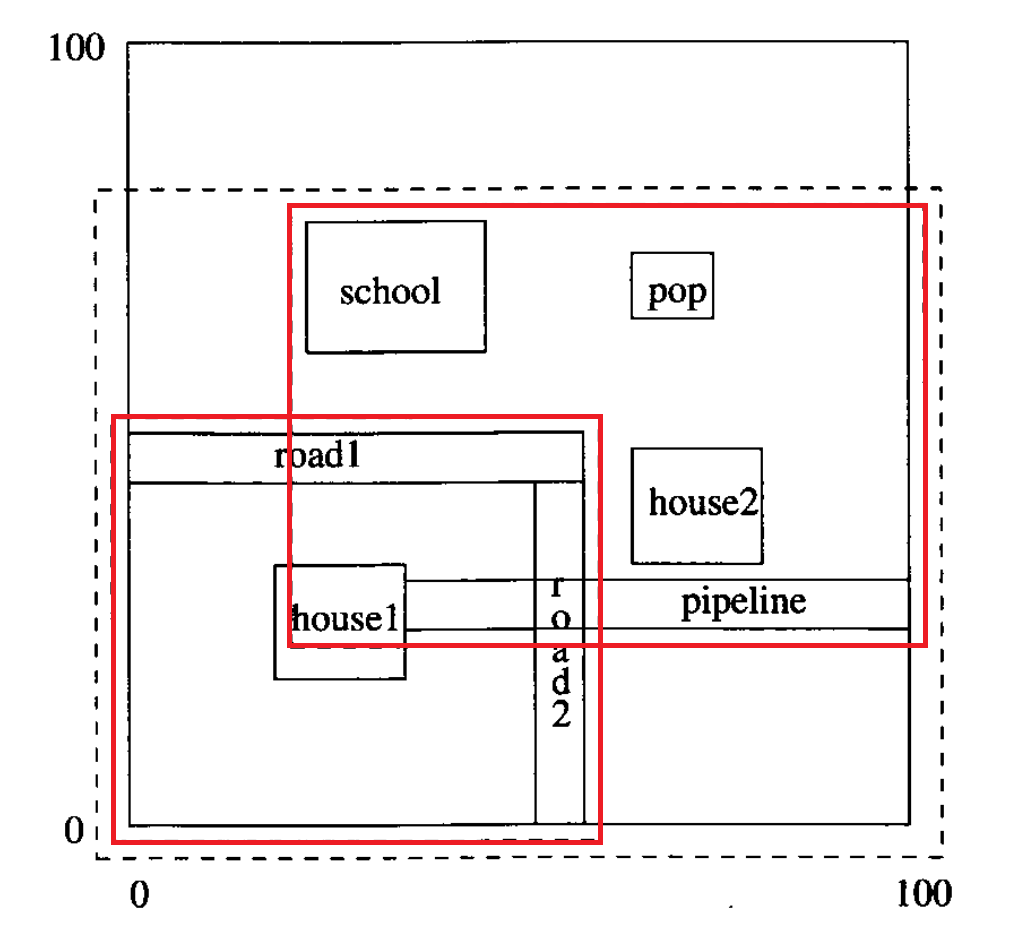
\includegraphics[width=0.6\linewidth]{handout/img/3-rtree2.png}
    \caption{rtree分层}\label{fig:3-rtree2}
\end{figure}

\subsection{rtree树}

rtree是一种空间索引数据结构，它模仿btree是一个多叉树，以固定大小的页面为节点。每个节点对应于一个区域，或者说是一个bounding box。rtree也分为根节点、内部节点、叶子节点。叶子结点上包含图元，其对应的矩为所有对象的外包矩形，非叶结点的矩形为所有子结点矩形的外包矩形。

\section{倒排索引}

在通常的应用中，我们使用key来访问索引，通过索引找到key对应的内容。倒排索引inverted index则相反，使用部分内容来找到包含该内容的所有key。

\begin{figure}[H]
    \centering
    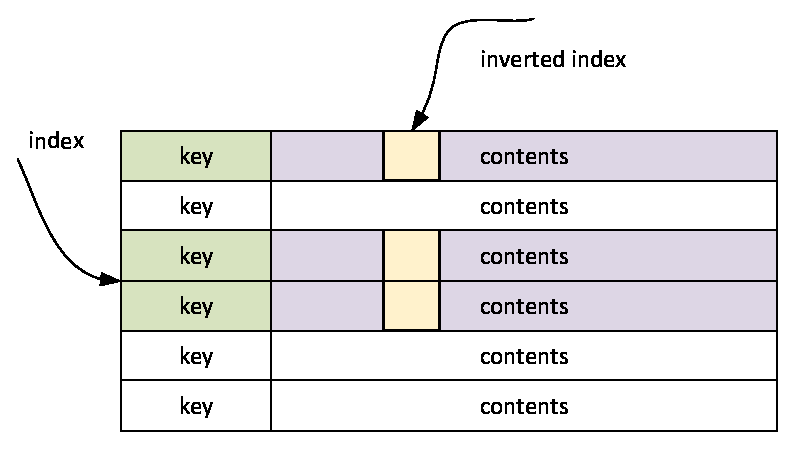
\includegraphics[width=0.6\linewidth]{handout/img/3-inverted.eps}
    \caption{倒排索引}\label{fig:3-inverted}
\end{figure}

倒排索引经常使用在全文检索中，例如搜索引擎。在搜索引擎中，用户输入一个查询字符串，搜索引擎需要找到包含该字符串的所有文档。倒排索引可以将每个文档中的每个单词作为key，将包含该单词的所有文档作为value，构建一个倒排索引。

\begin{exercise}
    搜索引擎的工作原理是怎样的？在搜索引擎中输入一个关键字，搜索引擎是象数据库一样即时查找的吗？
\end{exercise}

\subsection{标签}

在个人博客等应用中，经常对文章或者照片添加标签，例如“技术”、“生活”、“工作”等。用户可以根据标签来查找自己感兴趣的内容。标签索引就是用来支持这种功能的索引。

标签要看成对象的一种属性，根据标签来查找对象，实际上也是一种倒排索引，因为标签是对象的属性。但是标签应用中，并不需要象搜索引擎那么大型，因为标签的数量通常是比较少的，并且应用中很少有标签删除操作。

\subsubsection*{基于bitmap的标签系统}

将对象用id整型来表示，要构造标签索引，需要为每个标签维护一个bitmap，bitmap的每个位表示对应对象是否有该标签。id空间比较大，为了保存bitmap可以采用roaring压缩方案。

\begin{exercise}
    构思一个标签系统，支持添加标签、根据标签查找对象。
\end{exercise}

\subsubsection*{kv标签}

博客应用中，文章打的标签是tag类型。有些应用中，标签还可以带value，例如在iot设备中，某个检测点带的标签为position=32，意思是标签position的value值为32。